% !TEX root = ../tjumain.tex

\chapter{协议设计}

\section{总体设计}

为实现 TCP 的全部协议内容,我们将协议拆分成5个部分:连接建立、可靠数据传输、流量控制、连接关闭 以及 拥塞控制。在本章中,将从流程图和状态机的角度进行宏观描述,而代码实现将在下一章中进行详细介绍。

\section{连接建立的设计}

连接建立的流程设计如图\ref{fig:established}所示

\begin{figure}[!htbp]
    \centering
    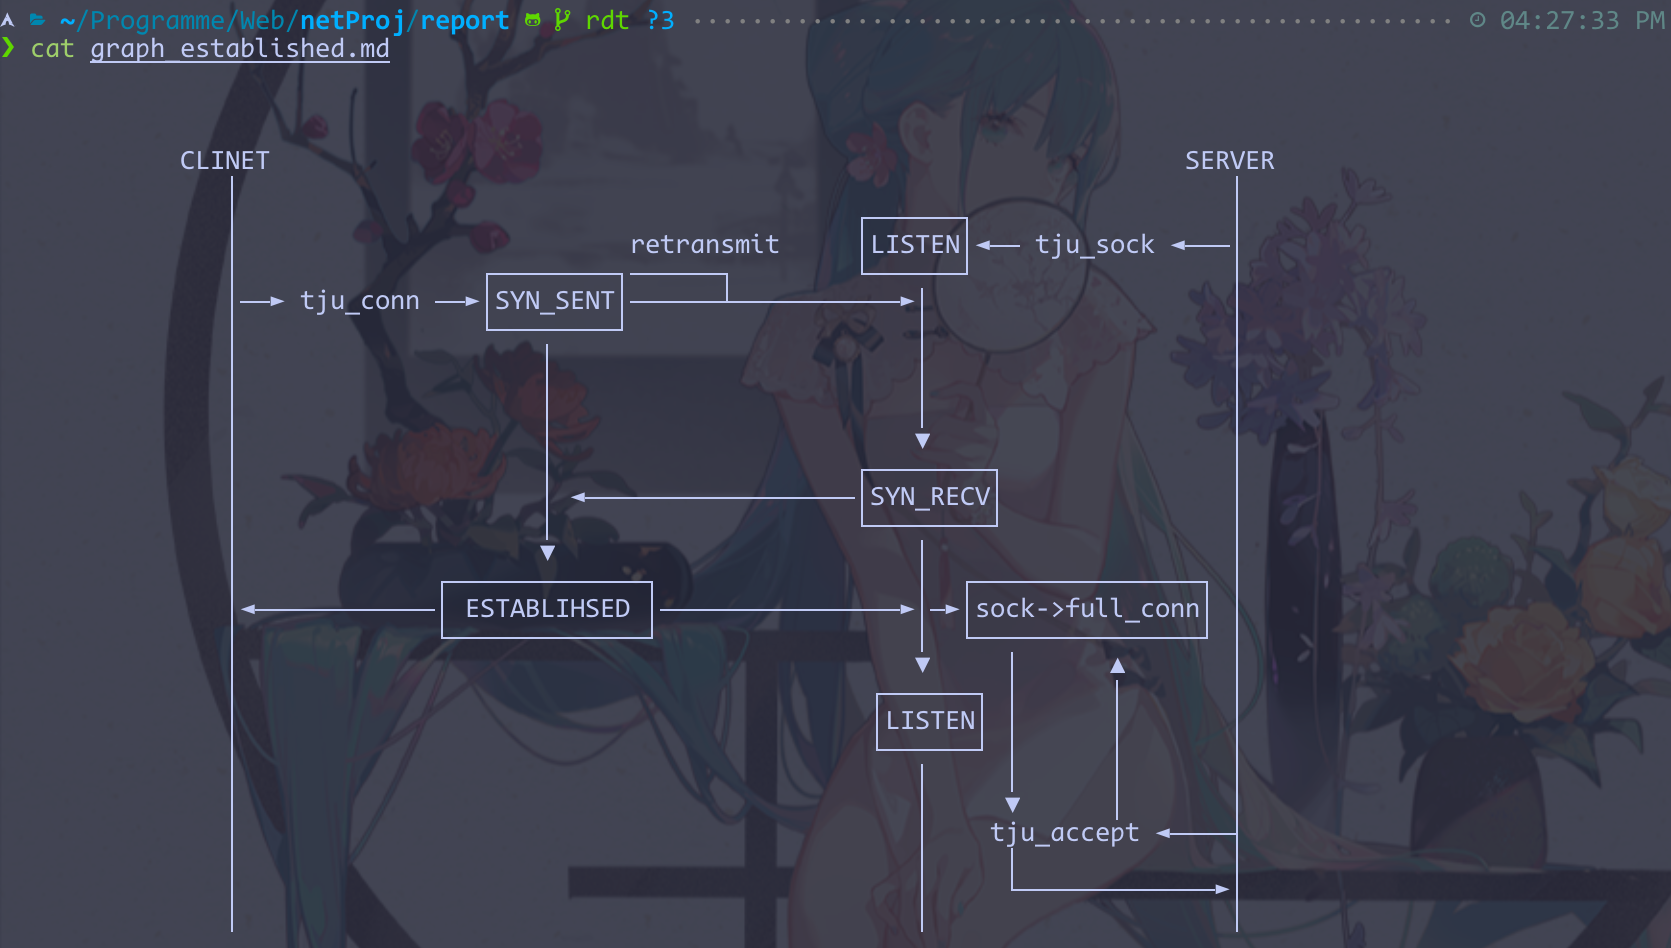
\includegraphics[width=1.0\textwidth]{established.png}
    \label{fig:established}\caption{连接建立流程图}
\end{figure}


由图可知,连接建立应当以 tju\_conn 和 tju\_accept 两个 API 供用户使用,(当然,首先server端需要使用 tju\_sock 接口获取一个初始的 socket)。

状态机如图\ref{fig:established_FSM}所示:

\begin{figure}[!htbp]
    \centering
    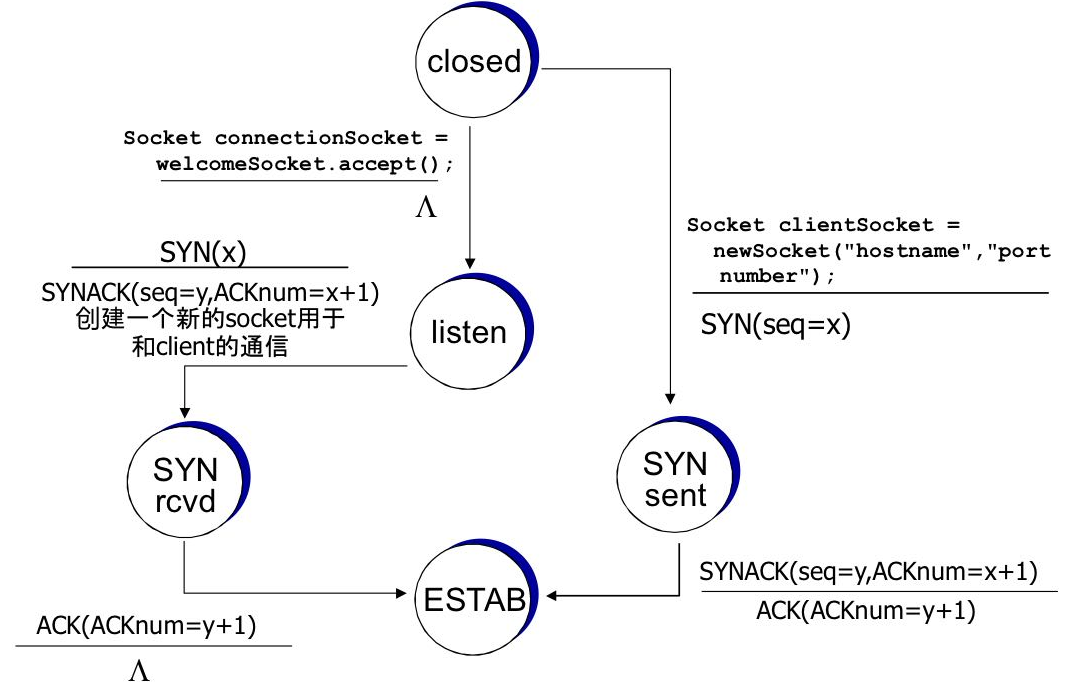
\includegraphics[width=1.0\textwidth]{established_FSM.png}
    \label{fig:established_FSM}\caption{连接建立 FSM}
\end{figure}

具体流程如下:
\begin{enumerate}
    \item Server 端使用 tju\_sock 接口获取一个处于 LISTEN 状态的 socket 
    \item Client 端调用 tju\_conn 接口向 Server 端发送报文1(请求连接),必要时进行超时重发(这个在后期会与 rdt 进行融合),并将自己的状态设置为 "SYN\_SENT"
    \item Server 端接受到报文1,确认要连接,发送报文2,并将自己的状态设置为 "SYN\_RECV"
    \item Client 端接收到报文2后,将自己的状态设置为 "ESTABLISHED" 并向上层接口返回一个建立连接的socket。同时,向 Server 发送报文3作为答复。
    \item Server 端接收到报文3后新建一个 socket 并将其放入初始 socket 的全连接队列中。
    \item 当 Server 端调用 tju\_accept 进行连接接收时,只需从 全连接队列中拿出一个即可。
\end{enumerate}

\section{可靠数据传输的设计}


可靠数据传输的流程图如图\ref{fig:rdt}所示:

\begin{figure}[!htbp]
    \centering
    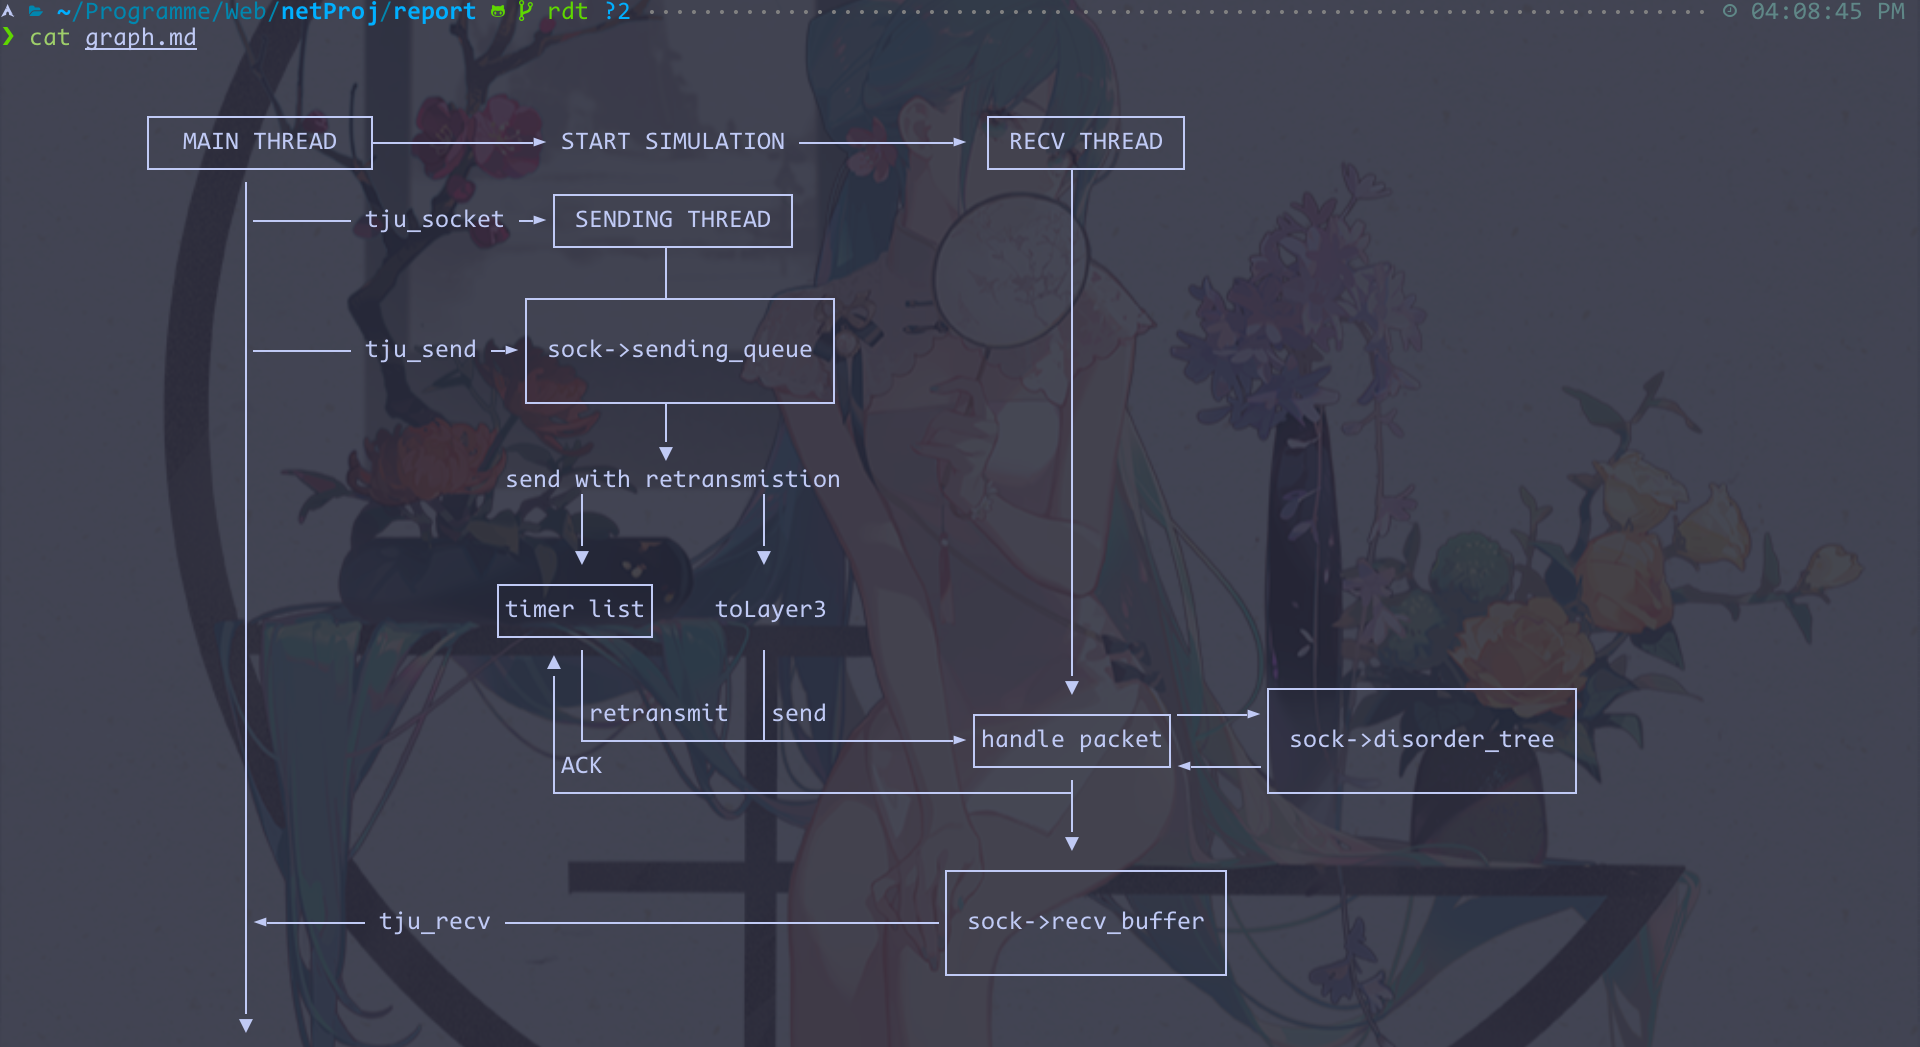
\includegraphics[width=1.0\textwidth]{rdt.png}
    \label{fig:rdt}\caption{可靠数据传输流程图}
\end{figure}

在该图中,我们通过 ACK 和 超时重传的原理进行环境丢包、接收端丢包的处理。为此我们需要实现一些数据结构:发送端负责超时重传的 timer\_list 以及 接收端负责接收乱序数据的 disoerder\_tree 缓冲区。

在发送端,我们直接采用了 sending\_queue 的结构将主线程和发送线程连接,即在 tju\_send 函数中,将数据打包成 tju\_packet\_t 结构,并放入sending\_queue,然后发送线程从 sending\_queue 中获取新的发送包裹。将数据以包为单位进行计数和重传,使得整个程序的可读性、可维护性提高。同时,我们设计并实现了自定义的队列数据结构,在“连接建立”中的全连接队列 和 “可靠数据传输” 的 发送队列使用(具体实现见下一章)。


\subsection{状态机设计}

在此,我们给出两个状态机的设计图,结合我们的流程图进行更加详细的设计阐述。

\subsubsection*{Client 端状态机设计}

\begin{figure}[!htbp]
    \centering
    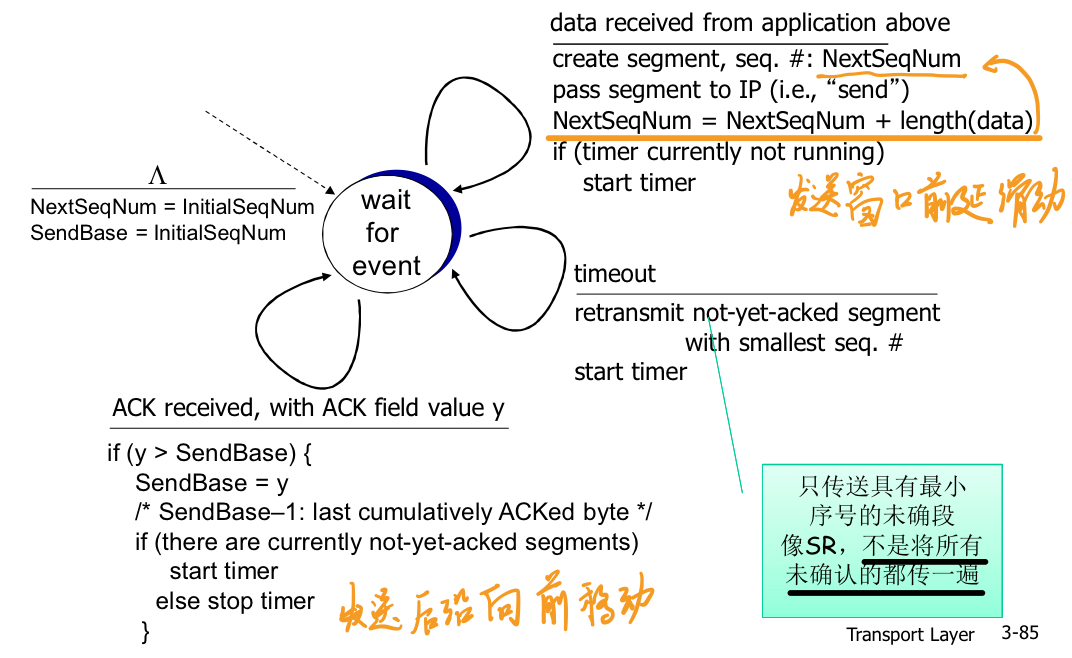
\includegraphics[width=1.0\textwidth]{figures/CLIENT_FSM.png}
    \label{fig:client_fsm}\caption{Client FSM}
  \end{figure}

Client 端状态机如图\ref{fig:client_fsm}所示。Client 端需要响应三种事件:

\begin{enumerate}
    \item 来自上层的调用,将数据打包并发送给下一层实体(toLayer3),然后新建 TIMER 并 注册之
    \item 来自TIMEOUT 通过 TIMER 的信息进行超时重传
    \item 收到 ACK,确认 ACK 的状态,根据 ACK 信息选择性地关闭 TIMER 
\end{enumerate}

\subsubsection*{Server 端状态机设计}

\begin{figure}[!htbp]
    \centering
    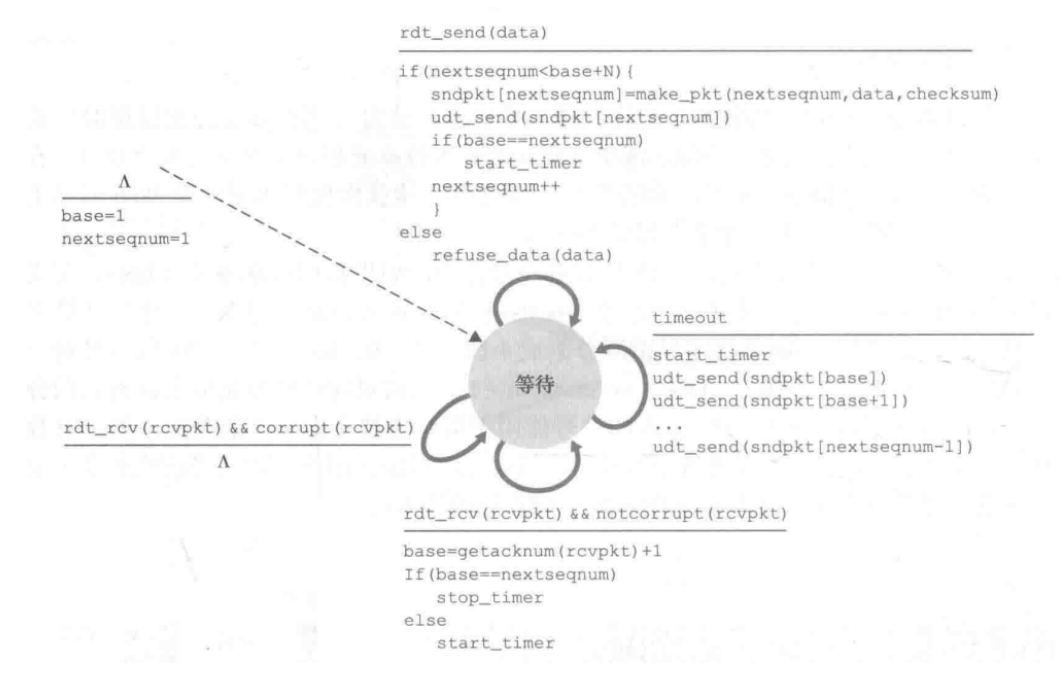
\includegraphics[width=1.0\textwidth]{figures/SERVER_FSM.png}
    \label{fig:server_fsm}\caption{Server FSM}
  \end{figure}

在 Server 端,我们目前暂不考虑数据出错的情况,即达到的包,都是正确的。在此情况下,我们需要处理一下情况:

\begin{enumerate}
    \item 到达SEQ正确:判断缓冲区大小,选择性的将其放入缓冲区,发送ACK。同时在AVL中递归地查找连续的正确的包裹
    \item 到达SEQ大了:将其放入 AVL Tree 并发送ACK
    \item 到达SEQ小了:收到过,丢弃
\end{enumerate}

\subsection{超时重传机制}

我们采用的是 ACK 累计确认型的超时重传机制,因此需要在 Server 端建立一个 AVL 类型的缓冲区,乱序接收包裹,顺序拿出包裹。

\paragraph*{连接建立时} 丢失有三种:第一次握手丢失,服务端返回第二次握手丢失,以及第三次确认丢失。第一、二个由 Client 端设置定时器保护,第三个由 Server 端设置定时器保护,即当收到第三次确认时,Server 端再将信息定时器进行关闭。

\paragraph*{发送数据时} 丢失有两种:发送数据丢失(Seq),发送ACK丢失。二者对于 Client 端的表现均是长时间(RTO)没收到 ACK 信息,于是我们将定时器设置在 Client 端,由 Client 端进行超时重传。而 Server 只对于前者,即发送数据丢失的情况作出反馈,即设置乱序到达,顺序提交的机制,确保因超时而呈现乱序到达的数据得以顺序提交给上层用户。

\subsubsection*{RTO 计算法则}

RTO 是超时重传机制的基础。由于网络变化,RTO应当是动态调整的。如果TCP 过早重传,会导致注入多数不必要的报文,阻塞网络。如果过晚重传,则会影响网络使用效率。我们根据 RFC793 的标准,让Socket维护了一个 SampleRTT均值(EstimatedRTT)通过如下公式进行更新:
\begin{equation}
    EstimatedRTT := (1-\alpha)\times EstimatedRTT + \alpha\times SampleRTT
\end{equation}\label{eq:est}

除了RTT,RFC 6298 还定义了 RTT 的偏差 DevRTT 的计算,用于usuan SampleRTT 和EstimatedRTT 的偏离程度
\begin{equation}
    DevRTT := (1-\beta)\times DevRTT + \beta\times|SampleRTT - EstimatedRTT|
\end{equation}
于是,最终的TRO计算公式如下:
\begin{equation}
    RTO := EstimatedRTT + 4\times DevRTT
\end{equation}\label{eq:rto}

\subsection{缓冲区与滑动窗口设计}

\paragraph*{发送端缓冲区与滑动窗口}

发送段共有 sending\_queue 和 timer\_list 两个数据结构组成发送缓冲区。采用 sending\_queue,队列的数据结构,上层将包裹放入sending\_queue表示要发送,发送线程读取 sending\_queue 来进行发送。然后利用 timer\_list 的个数确定滑动窗口的大小。即,使用 timer\_list 来代表进入滑动窗口的包裹,通过发送将其放入 timer\_list,通过 ACK 将其踢出。于是,sending\_queue 实际表示在缓冲区且不在滑动窗口的部分。滑动窗口的大小以 segment 计数。

\paragraph*{接收端缓冲区}

接收端有两个缓冲区,一个是正序到达时直接放入的 recv\_buf,共 tju\_recv 调用获取。另一个是手动实现的 AVL 树,能够快速插入乱序数据并正序取出,用于存入乱序到达的包裹。



\section{流量控制的设计}

流量控制也是 TCP 标准功能之一,是构成可靠传输的关键步骤,能够与其他 TCP 实体一起,维护整个网络的传输可靠性。如果流量过大,则会导致接收方不断丢弃传输的结果,发送方不断进行重发。故而,Server 端需要将rwnd的信息通过 ACK 信息携带给 Client 端,让 Client 能够正确地调整发送速率。

具体来说,我们在 Server 端的 handle\_packet 函数中加入对当前接收窗口更新的代码:接收到按顺序达到的包裹、将数据放入 recv\_buf 时更新rwnd值。同时在 tju\_recv 函数中,上层拿走数据时也进行更新。同时,我们在返回 ACK 时,将 rwnd 信息通过 advertise 字段返回给 Client 端。当然,我们需要首先约定一个 Window\_Dlen,这样在描述 rwnd 时,只需描述其 segment 的大小。

在 Client 端,我们通过在发送线程中 "send with retransmission" 时先对当前 swnd 和 对方 rwnd 的大小进行比较,如果大于,则等待 rwnd 变大或 swnd 因为 ACK 而减少时再发送包裹。此处我们因为引入了 timer\_list,于是只需要使用 timer\_list 的个数作为 swnd 即可。同时,我们需要在接收到 ACK 时对当前 rwnd(对方的) 数值进行更新。


\section{连接关闭的设计}

我们的协议应当给出API tju\_close 让上层进行调用。我们需要明确的是,当且仅当socket两端都调用了 tju\_close,我们才能认为该 socket 已经被关闭了,可以回收了。否则 socket 的接收功能依旧要工作。且处于当前重传 buffer 中的包裹必须全部完成。

连接关闭的FSM图如图\ref{fig:close_fsm}所示:

\begin{figure}[!htbp]
    \centering
    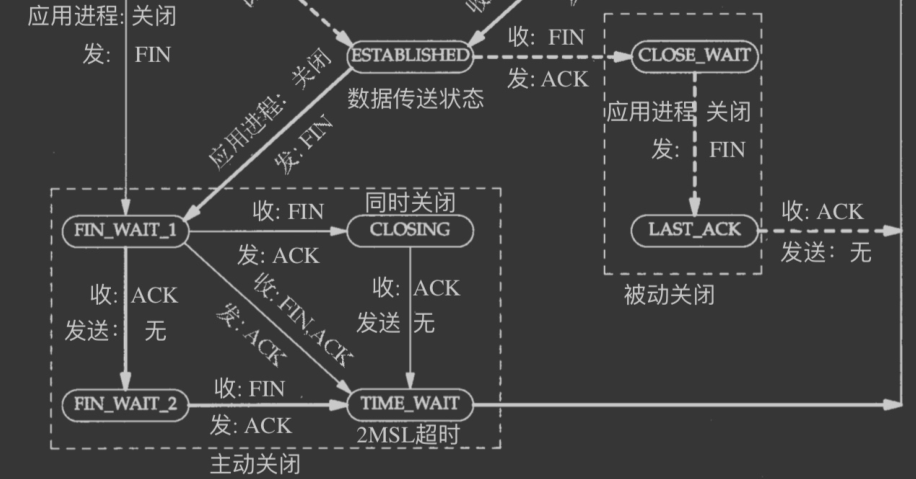
\includegraphics[width=1.0\textwidth]{close_FSM.png}
    \label{fig:close_fsm}\caption{连接关闭 FSM}
  \end{figure}

在此我们对关闭时的两种情况进行描述:

\subsection*{一方发起关闭}

其实由于 TCP 协议的设计时的对等性考虑,并没有 Client 或 Server 端的区分,在此,我们为了方便进行讨论,使用 Client 端表示优先调用 tju\_close 的一方,Server 作为后调用 tju\_close 的一方。

Client 端首先调用 tju\_close 后,将状态转换为 "FIN\_+WAIT\_1" ,并将一个 FIN 包放入自己的 sending\_queue 中,等待发送线程进行超时重传型的发送。同时,拒绝上层继续向 sending\_queue 中放入包裹,但需要将此时 sending\_queue 以及 timer\_list 中的包裹全部安全送达。等待对方的ACK使得自己能够进入 "FIN\_WAIT\_2" 状态。然后继续等待,直到对方发送了 FIN 包、我方完成所有超时重传任务时,我方状态变为 CLOSED,并销毁 socket。

Server 端接收到 FIN 包时,将自己的状态变为 CLOSE\_WAIT 并返回一个 ACK,但仍然保持接收和发送功能。直到我方调用 tju\_close 进入关闭程序:将己方状态转换为 "LAST\_ACK" 并拒绝上层继续向 sending\_queue 中放入任何包裹,但需要将已经在 sending\_queue 和 timer\_list 中的包裹进行重传型的发送,安全送达对岸,即使对面已经宣布关闭。在接受到对方发送的关于 FIN 包裹的 ACK 时,我们才能关闭己方socket。因为如果对方能够对 FIN 包裹进行 ACK,由于我们采用的是累计确认,则此时代表FIN包裹发送之前所有的包裹都已经收到。完成了对上层的承诺,可以关闭了。

\subsection*{两方同时关闭}

此时我们认为是 Server 端在没有接收 FIN 包,且 Client 端已经发送的情况下发送了 Server 端的 FIN 包裹。

此时 Server 和 Client 端在接收到 FIN 包裹时,其状态都是 "FIN\_WAIT\_1",由于尚未接收到 ACK 而直接接收到了 FIN,故而将状态转变为 ”TIME\_WAIT" 并在两个超时后直接关闭连接。由于此时接收到了 FIN(累计确认) 且自己已经发送 FIN,故而表明我们没有继续发送包裹,且对方亦然,所有包裹都已经发送、接收完毕,该 socket 可以关闭。

\section{拥塞控制的设计}

在拥塞控制中,我们采用一个 cwnd 的结构进行控制,在发送线程每次从 sending\_queue 读取包裹时,首先需要根据当前的 rwnd 更新 滑动窗口的大小,在包含拥塞控制的设计中,我们使用加入对 cwnd 的考量,即选取当前 cwnd 和 rwnd 中较小的一个作为当前 swnd 的值。然后根据 swnd 来判断是否在该轮循环中进行数据的发送。

cwnd 的更新,为此,我们创建一个cwnd 的数据结构,包括当前 cwnd 的状态 cwnd\_STATE 和窗口大小 cwnd,上限 sshresh ,并在以下事件结点进行更新:

\begin{enumerate}
    \item 新的ACK:按照状态进行更新,同时按照情况将状态从慢启动换为拥塞避免
    \item 出现超时:将 cwnd 降为1,sshresh 降为 cwnd / 2 + 1,同时设置状态为拥塞避免
    \item 出现三个连续ack: 将 cwnd 将为 1/2 + 3,sshresh 将为 cwnd / 2 + 1,同时将状态设置为慢启动
\end{enumerate}

拥塞控制的FSM如图\ref{fig:cwnd_FSM}所示


\begin{figure}[!htbp]
    \centering
    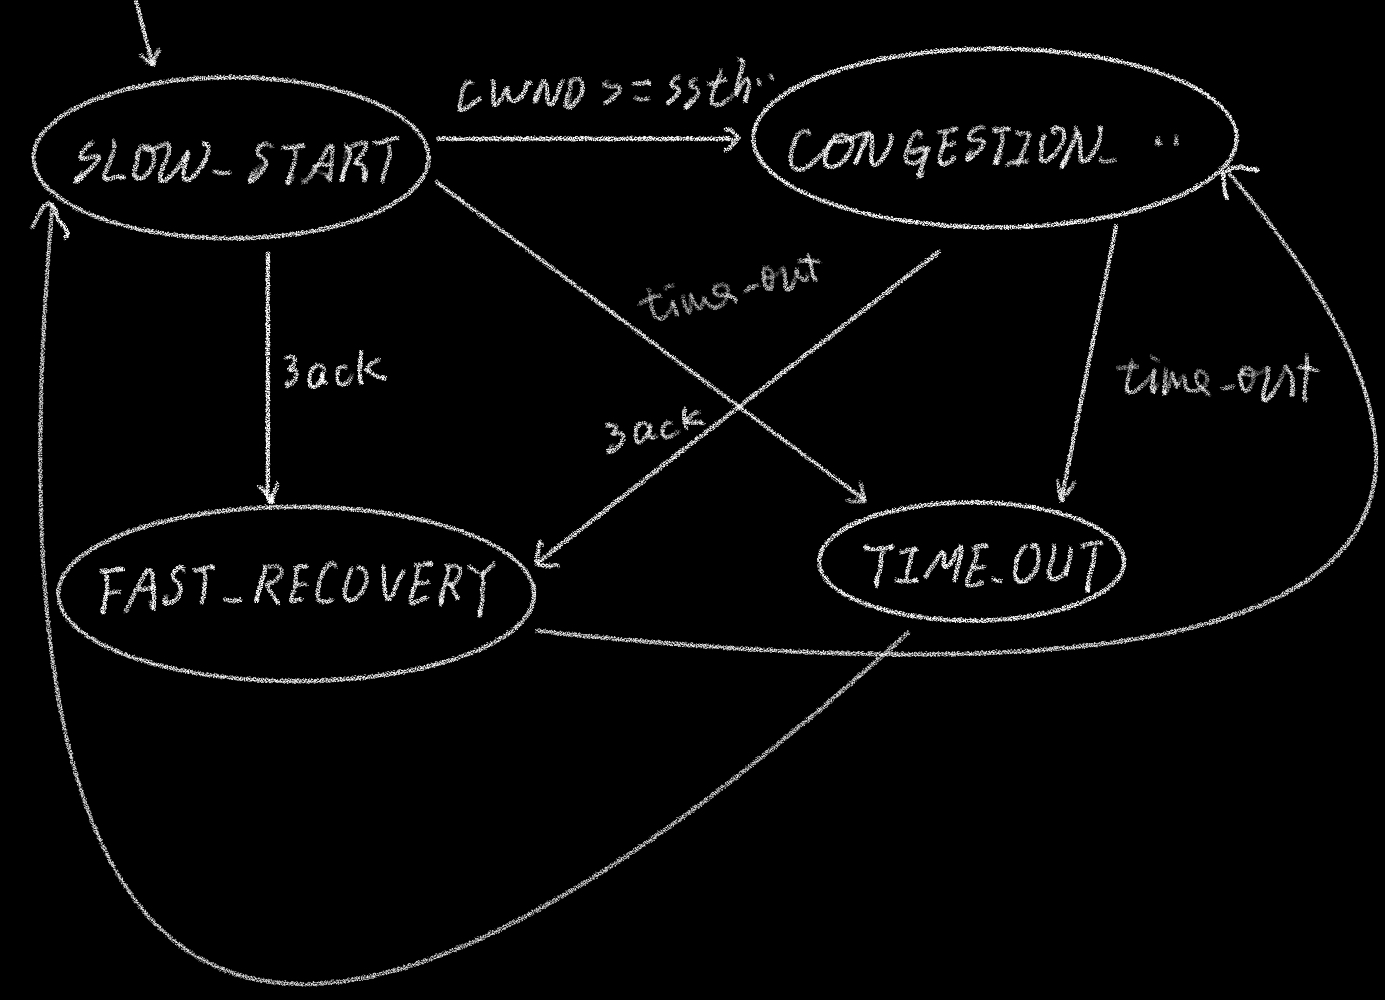
\includegraphics[width=0.8\textwidth]{cwnd_FSM.png}
    \label{fig:cwnd_FSM}\caption{拥塞控制 FSM}
  \end{figure}



